\documentclass{article}

\usepackage{graphicx}

\title{Compte Rendu HashTable}
\date{2024-02-19}
\author{Wilhem Blondel et Alexandre Genin}

\begin{document}
    \pagenumbering{gobble}
    \maketitle
    \newpage
    \pagenumbering{arabic}

    \section{Section}    
    Hello World!

    \begin{figure}
        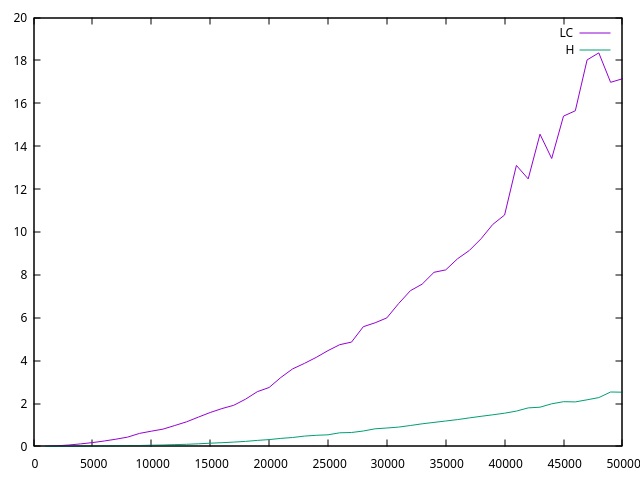
\includegraphics[width=\linewidth]{graph.png}
        \caption{Recherche de doublons entre une liste chaînée et une table de hachage de taille 20}
        \label{fig:graph20}
    \end{figure}

    Le graphe \ref{fig:graph20} montre le truc bidule chouette
        
\end{document}
